\section{Benchmarks}
\label{app:benchmarks}

Below, we provide a more elaborate description of (construction of) the benchmarks we consider in our work.
A summary of their statistics can be found in \cref{tab:dataset}.

\begin{table}
\centering
\begin{tabular}{c|c|c}
    Benchmark & \# Samples & \# labels \\
    \hline
    ANLI & 1200 & 3 \\
    HANS & 30000 & 2 \\
    MNLI & 9815 & 3 \\
    SNLI & 9842 & 3 \\
    $\alpha$NLI & 1532 & 2 \\
\end{tabular}
\caption{Dataset details}
\label{tab:dataset}
\end{table}

\subsection{SNLI}
Introduced by \citet{bowman-etal-2015-large}, the Stanford Natural Language Inference (SNLI) dataset was one of the first large-scale NLI dataset for NLP evaluation.
The dataset comprises of 570K human-authored English sentence pairs, sourced by asking Amazon Mechanical Turk workers to supply hypotheses for the three labels available in the dataset -- entailment, neutral and contradiction -- given a premise comprised by an image caption drawn from a pre-existing corpus.
For 57K of the resulting samples were then labeled by four additional annotators.
In this work, we consider the 10K development set of the corpus.
Like the original paper, we exclude samples for which no gold label exists because there was no label that three or more annotators agreed on.

\subsection{MNLI}
The Multi-Genre NLI (MNLI) corpus \citep{williams-etal-2018-broad} was introduced as an alternative to SNLI that captures more genres and more challenging examples, representing both written and spoken speech in a range of different styles, degrees, formalities, and topics.
The data collection procedure of the corpus is similar to the SNLI procedure both in terms of sourcing and validation.
Unlike SNLI, the MNLI premise sentences are derived from nine different sources, aiming to represent the full range of American English rather than a single image captioning corpus.
As for SNLI, we consider the validation corpus of the dataset and exclude samples that have no gold label.

\subsection{HANS}
Deviating from previous datasets, the adversarial dataset Heuristic Analysis for NLI Systems \citep[HANS,][]{mccoy-etal-2019-right} is not crowd-sourced, but synthetically generated using templates.
Specifically, the templates are designed to generate examples that can not be solved through heuristics such as lexical, subsequence, or constituent overlap.
At the time of proposal, none of the SOTA models were able to solve such examples.

\subsection{ANLI}
The second adversarial dataset we consider is Adversarial NLI \citep[or ANLI,][]{nie-etal-2020-adversarial}.
The dataset, created with the primary aim to make SOTA models fail, is sourced iteratively in a human-in-the-loop setup.
Given a premise and a target label, annotators are asked to propose hypotheses that may fool models.
The produced samples are then tested on a model, and the examples that do indeed receive an incorrect label are re-validated by one or more human validators.
The dataset consists of three sets of increasingly challenging examples, where in each round more powerful models are considered that are trained on examples from the previous round.
The third round furthermore contains a set of more diverse premises.
For our experiments, we are using the dev set of round 3, the most challenging set of the benchmark.

\subsection{$\alpha$NLI}
Differing in setup from the previously described benchmarks, $\alpha$NLI or abductive NLI \citep{bhagavatula2020abductive} focuses on \emph{abductive reasoning} -- which they describe as the inference of the most plausible explanation for an incomplete observation.
The samples in $\alpha$NLI consist of a pair of observations at two consecutive times, and a plausible hypothesis that explains tho two observations, and an implausible hypothesis that does not (or to a lesser extent).
The task is to select the most plausible hypothesis.
To construct the data \citet{bhagavatula2020abductive} first draw observation pairs from a stories dataset and then ask crowd-sources to generate plausible and implausible hypotheses. 
For each observation pair, multiple plausible and implausible hypotheses are crowd-sourced, and adversarial filtering is applied to retain one challenging pair of hypotheses.
We use the development set of the corpus for our experiments.



\section{Entropy vs accuracy plots}\label{app:entropy_vs_accuracy}

In addition to \cref{fig:entropy_accuracy} highlighting the results on the Llama-3.1 8B and 405B models, we also show the accuracy vs entropy plots of all other models we use for our analysis: Llama-3.1 70B, Mistral 7B, Mixtral 8x7B, and Mixtral 8x22B in \cref{fig:entropy_accuracy_all}. The Mistral family of models also show a similar trend where larger models have lower accuracies for higher entropy buckets.

\begin{figure*}[t]
    \centering
    \begin{subfigure}[b]{0.23\textwidth}
        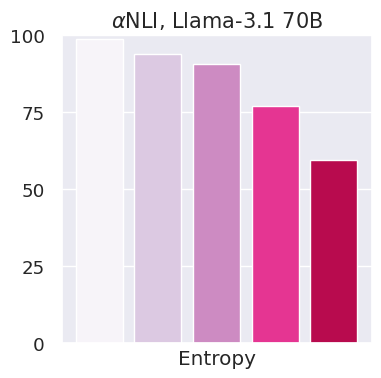
\includegraphics[height=3.6cm]{figures/appendix/entropy_acc_abductivenli_70B}
        % \caption{}
    \end{subfigure}
    \begin{subfigure}[b]{0.23\textwidth}
        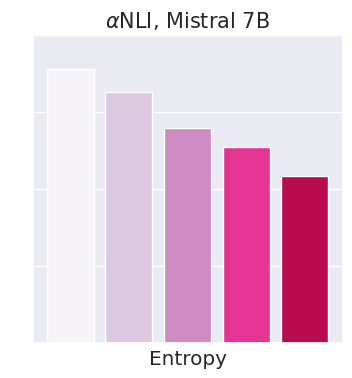
\includegraphics[height=3.6cm]{figures/appendix/entropy_acc_abductivenli_7B}
        % \caption{}
    \end{subfigure}
    \begin{subfigure}[b]{0.23\textwidth}
        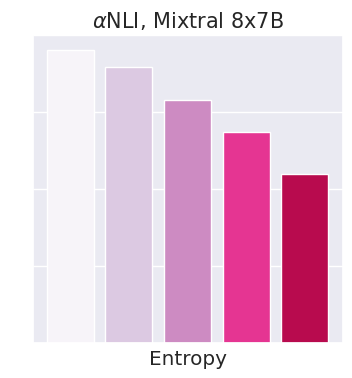
\includegraphics[height=3.6cm]{figures/appendix/entropy_acc_abductivenli_8x7B}
        % \caption{}
    \end{subfigure}
    \begin{subfigure}[b]{0.23\textwidth}
        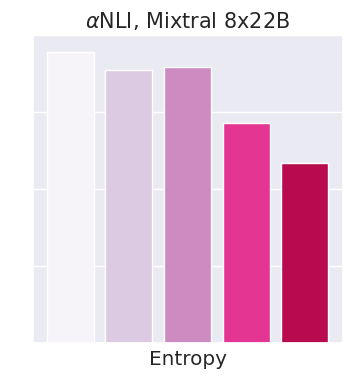
\includegraphics[height=3.6cm]{figures/appendix/entropy_acc_abductivenli_8x22B}
        % \caption{}
    \end{subfigure}\\
    \begin{subfigure}[b]{0.23\textwidth}
        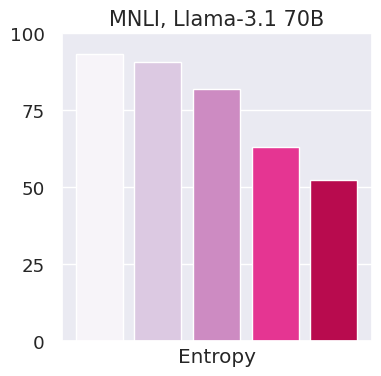
\includegraphics[height=3.6cm]{figures/appendix/entropy_acc_mnli_matched_70B}
        % \caption{}
    \end{subfigure}
    \begin{subfigure}[b]{0.23\textwidth}
        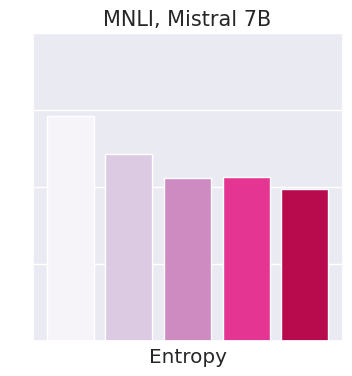
\includegraphics[height=3.6cm]{figures/appendix/entropy_acc_mnli_matched_7B}
        % \caption{}
    \end{subfigure}
    \begin{subfigure}[b]{0.23\textwidth}
        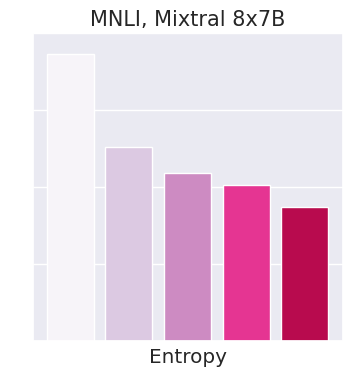
\includegraphics[height=3.6cm]{figures/appendix/entropy_acc_mnli_matched_8x7B}
        % \caption{}
    \end{subfigure}
    \begin{subfigure}[b]{0.23\textwidth}
        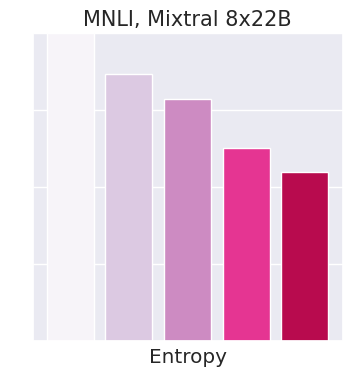
\includegraphics[height=3.6cm]{figures/appendix/entropy_acc_mnli_matched_8x22B}
        % \caption{}
    \end{subfigure}\\
    \begin{subfigure}[b]{0.23\textwidth}
        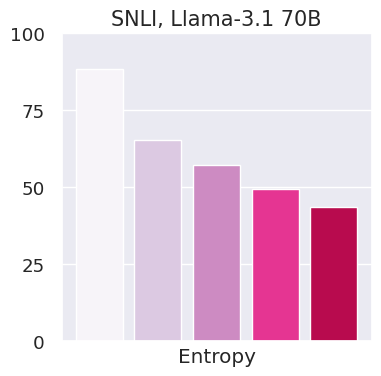
\includegraphics[height=3.6cm]{figures/appendix/entropy_acc_snli_70B}
        % \caption{}
    \end{subfigure}
    \begin{subfigure}[b]{0.23\textwidth}
        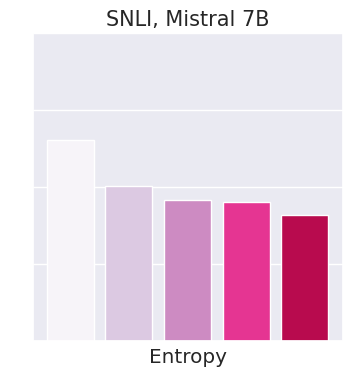
\includegraphics[height=3.6cm]{figures/appendix/entropy_acc_snli_7B}
        % \caption{}
    \end{subfigure}
    \begin{subfigure}[b]{0.23\textwidth}
        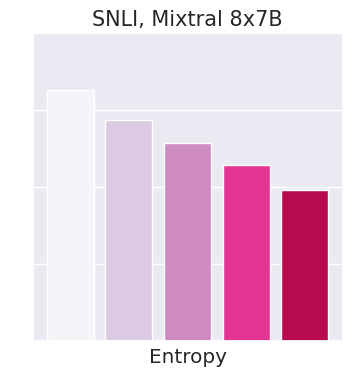
\includegraphics[height=3.6cm]{figures/appendix/entropy_acc_snli_8x7B}
        % \caption{}
    \end{subfigure}
    \begin{subfigure}[b]{0.23\textwidth}
        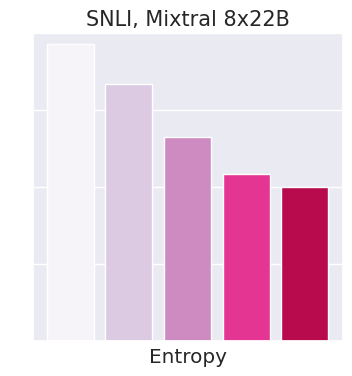
\includegraphics[height=3.6cm]{figures/appendix/entropy_acc_snli_8x22B}
        % \caption{}
    \end{subfigure}
    \caption{\textbf{Accuracy versus entropy.} We show how the accuracy of Llama-3.1 70B and the Mistral series of models changes as the entropy of the human label distributions increases.}
    \label{fig:entropy_accuracy_all}
\end{figure*}

\section{Prompt templates}

The prompt templates used for each task are presented in \cref{tab:prompt_template}.

\begin{table*}[t]
    \centering
    \small
    \begin{tabular}{lp{8cm}}
        \toprule
        \textbf{Benchmark} & \textbf{Prompt Template} \\
        \midrule
        MNLI, SNLI, ANLI & \begin{verbatim}

Premise: {{ x["premise"] }}
Hypothesis: {{ x["hypothesis"] }}
A. Entailment
B. Neutral
C. Contradiction
Answer: {{ x["answer"] }}


Premise: {{ premise }}
Hypothesis: {{ hypothesis }}
A. Entailment
B. Neutral
C. Contradiction
Answer: {{ choice_text }}
\end{verbatim} \\
\midrule
AbductiveNLI & \begin{verbatim}

Observation 1: {{ x["obs1"] }}
Observation 2: {{ x["obs2"] }}
A. {{ x["choices"]["A"] }}
B. {{ x["choices"]["B"] }}
Answer: {{ x["answer"] }}


Observation 1: {{ obs1 }}
Observation 2: {{ obs2 }}
A. {{ choices["A"] }}
B. {{ choices["B"] }}
Answer: {{ choice_text }}
\end{verbatim} \\
\midrule
HansNLI & \begin{verbatim}

Premise: {{ x["premise"] }}.
Hypothesis: {{ x["hypothesis"] }}.
A. Entailment
B. Non-Entailment
Answer: {{ x["answer"] }}


Premise: {{ premise }}.
Hypothesis: {{ hypothesis }}.
A. Entailment
B. Non-Entailment
Answer: {{ choice_text }}
\end{verbatim} \\
\bottomrule
\end{tabular}
\caption{Prompt Templates for each task}
\label{tab:prompt_template}
\end{table*}

